\noindent{\bf Directions:}
Circle the best answer.

\large

\newcommand{\columnbreak}{{\par\vfill\null\pagebreak[4]}}

% the \columnbreak macro is provided to easily skip to the next column

\medskip\hrule
\begin{enumerate}
  \item Wrap both sides of Taylor's rule with the exponential function;
        then, compute the Taylor's Series of $e^{ix}$ centered at $x=\pi^*$
        and create a polynomial expansion with 4 terms for $e^i$. This
        polynomial expansion can best be expressed by which of the following
        expressions?
        \begin{enumerate}
          \item $\displaystyle \sum_{n=0}^{\infty} (-1)^n \dfrac{x^n}{n!}$
          \item $\displaystyle \MultiIntegral{3} x^3 e^x \differential x$
          \item $e^{2 \pi i k} - e^{2 \pi i (k + 1)}$
          \item $\displaystyle\sum_{n=-\infty}^{\infty} a_n \int_\gamma (z - z_0)^n \differential z$
        \end{enumerate}


  \item In order for Goldman Sachs to most effectively launder
        Malaysia's \textsc{1MDB} sovereign wealth fund, what economic policy
        would be best?
        \begin{enumerate}
          \item Lower the reserve requirement for foreign banks
          \item Increase the reserve requirement for foreign banks
          \item Lower the reserve requirement for domestic banks
          \item Increase the reserve requirement for domestic banks
        \end{enumerate}

  \item If Biden authorizes a \textsc{SWIFT} international banking
        transaction to launder money from Burisma in Ukraine to a hedge
        fund in Washington, D.C., it is an example of which of the
        following types of governmental economic involvement?
        \begin{enumerate}
          \item Open-market operations
          \item Reserve ratio
          \item Discount rate
          \item Government spending
        \end{enumerate}


        % you can also add context to a problem, like this:
        \vspace{0.5cm}

        In 2020, researchers at the University of California, Berkeley
        developed a new margin-based Condorcet voting algorithm called
        Split Cycle, which avoids common pitfalls associated with
        Condorcet voting methods such as ``spoiler effects'' and
        ``strong no show paradoxes''~\cite{splitcycle}.

        \bigskip

        \begin{figure}[h]
          \centering
          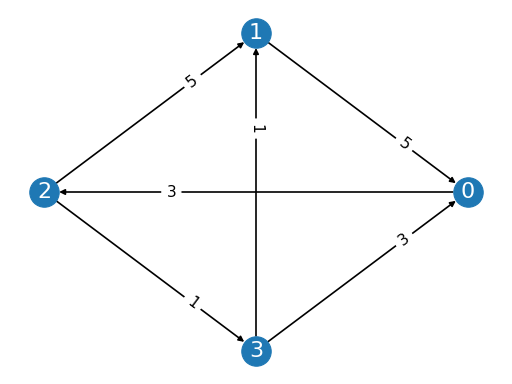
\includegraphics[width=0.4\textwidth]{assets/splitcycle.png}
          \label{}
          \caption{Voting margins graph}
        \end{figure}

        % columnbreak is a custom (user defined) macro that skips
        % to the next column
  \columnbreak

  \item Consider the voting margins matrix above.
        % Define colors for Python syntax highlighting
\definecolor{codegreen}{rgb}{0,0.6,0}
\definecolor{codegray}{rgb}{0.5,0.5,0.5}
\definecolor{codepurple}{rgb}{0.58,0,0.82}
\definecolor{backcolour}{rgb}{0.95,0.95,0.92}

% Define Python language settings
\lstdefinestyle{pythonstyle}{
  backgroundcolor=\color{backcolour},
  commentstyle=\color{codegreen},
  keywordstyle=\color{magenta},
  numberstyle=\tiny\color{codegray},
  stringstyle=\color{codepurple},
  basicstyle=\ttfamily\footnotesize,
  breakatwhitespace=false,
  breaklines=true,
  captionpos=b,
  keepspaces=true,
  numbers=left,
  numbersep=5pt,
  showspaces=false,
  showstringspaces=false,
  showtabs=false,
  tabsize=2
}

\lstset{style=pythonstyle}

\begin{lstlisting}[language=Python, caption=Calling Split Cycle from Python]
from pref_voting.margin_based_methods import split_cycle

split_cycle.display(mg)
\end{lstlisting}


        The above code will run the split cycle algorithm on the margin
        graph. Who will the Condorcet winners be?

        \begin{enumerate}
          \item $\begin{Bmatrix} 2 & 3 \end{Bmatrix}$
          \item $\begin{Bmatrix} 0 & 2 \end{Bmatrix}$
          \item $\begin{Bmatrix} 1 & 3 \end{Bmatrix}$
          \item $\begin{Bmatrix} 2 & 1 \end{Bmatrix}$
        \end{enumerate}
\end{enumerate}
